\documentclass[12pt]{article}

\usepackage{listings}
\usepackage{graphicx}
\usepackage{float}
\usepackage{hyperref}
\usepackage{ifthen}

\usepackage{amssymb} 
\usepackage{amsmath}
\usepackage{amsthm}
\usepackage{sansmath}
\usepackage{epsfig}

\usepackage[T1]{fontenc}
\usepackage{lmodern}
\renewcommand*\familydefault{\sfdefault}

\usepackage[margin=2cm]{geometry}

\usepackage[parfill]{parskip}
\linespread{1.2} 

\usepackage{xcolor}

\lstdefinestyle{code}{  
    commentstyle=\color{gray},
    keywordstyle=\color{blue},
    numberstyle=\tiny\color{gray},
    stringstyle=\color{teal},
    ndkeywordstyle=\color{purple},
    basicstyle=\ttfamily\footnotesize,
    breakatwhitespace=false,         
    breaklines=true,                 
    captionpos=t,                    
    keepspaces=true,                 
    numbers=left,                    
    numbersep=8pt,                  
    showspaces=false,                
    showstringspaces=false,
    showtabs=false,                  
    tabsize=4,
    frame=single,
    breaklines=true
}

\lstset{style=code}

\newcounter{question}
\setcounter{question}{1}
\newcounter{subquest}

\newcommand{\question}[1]{
    \stepcounter{question} 
    \ifnum\value{question}>1 \fi
    \vspace{.5em}
    \textbf{ \Large\thequestion \ - #1} \\
    \vspace{.5em} 
    \hrulefill \\
    \setcounter{subquest}{0}\ }

\newcommand{\subquestion}[1][true]{
    \stepcounter{subquest} 
    \ifthenelse{\equal{#1}{true} \and \value{subquest}>1}{\newpage}{}
    \vspace{1em}
    \textbf{\large Question \thequestion.\thesubquest}
    \vspace{.5em}\ \\}

\newcommand{\solution}
    {\hrulefill \par\vspace{0.5em}\noindent\emph{Solution.}\ }
    {\par\vspace{1em}}

\newcommand{\startappendix}{%
    \newpage
    \vspace{1em}
    {\Large\textbf{Appendix}}

    The complete code used for this assignment is provided in the appendix for reference. Files can be accessed directly at this \href{https://github.com/sjsusu/numerical_analysis}{GitHub repository}.
}

\usepackage{fancyhdr}
\setlength{\headheight}{15pt}
\pagestyle{fancy} 
\lhead{Math 5335: \emph{Numerical Analysis}}
\rhead{Homework 1}
\cfoot{}
\rfoot{}

\begin{document}
\question{Implement RK4}
Use baseline timestep $\Delta t = 0.01$ and $T=50$.
\begin{itemize}
    \item[a.] Run code with $\Delta t, \Delta t/2, \Delta t/4$.
    \item[b.] Plot $x(t)$ for each run on the same graph. Comment on convergence with decreasing $\Delta t$.
    \item[c.] Use built-in ODE solver and compare results.  
\end{itemize}

\solution

The following code was used to implement RK4 and run comparison with SciPy's built-in ODE solver, \texttt{solve\_ivp} (similar to MATLAB's \texttt{ode45}):

\begin{lstlisting}[language=Python, caption={Question 2 Python}]
import numpy as np
import matplotlib.pyplot as plt
from scipy.integrate import solve_ivp

def F(u, sigma, rho, beta):
    x, y, z = u
    dxdt = sigma * (y - x)
    dydt = x * (rho - z) - y
    dzdt = x * y - beta * z
    return np.array([dxdt, dydt, dzdt])

def RK4_step(u, h, sigma, rho, beta):
    k1 = F(u, sigma, rho, beta)
    k2 = F(u + (h / 2) * k1, sigma, rho, beta)
    k3 = F(u + (h / 2) * k2, sigma, rho, beta)
    k4 = F(u + h * k3, sigma, rho, beta)

    y_new = u + (h / 6) * (k1 + 2 * k2 + 2 * k3 + k4)
    return y_new
    
def RK4_solver(u_0, h, sigma, rho, beta, T=50):
    num_steps = int(T / h)
    u_values = np.zeros((num_steps + 1, len(u_0)))
    u_values[0] = u_0

    for n in range(num_steps):
        u_values[n + 1] = RK4_step(u_values[n], h, sigma, rho, beta)

    return u_values

if __name__ == "__main__":
    # < Some Styling Setup and Enable Latex >
    # ...
    # Use default parameters for Lorenz system (Case C)
    sigma, rho, beta = 10, 28, 8/3
    u_0 = np.array([1, 1, 1])
    dt = 0.01
    time_steps = [dt, dt/2, dt/4]
    
    # Run RK4 solver for each time step and plot results
    for h in time_steps:
        u_values = RK4_solver(u_0, h, sigma, rho, beta)
        time_values = np.arange(0, 50 + h, h)
        plt.plot(time_values, u_values[:, 0], label=rf"$\Delta t = {h}$")
    plt.xlabel(r"$t$")
    plt.ylabel(r"$x(t)$")
    plt.title("RK4 Results")
    plt.legend()
    plt.savefig('./outputs/rk4_q2.png', dpi=300)
    plt.cla()
    
    # Compare with SciPy's ODE solver
    scipy_solution = solve_ivp(
        lambda t, u: F(u, sigma, rho, beta), 
        [0, 50], 
        u_0, 
        t_eval=np.arange(0, 50 + dt, dt)
    )
    
    # Plot Scipy solution
    plt.plot(scipy_solution.t, scipy_solution.y[0], label="Scipy", color=default_colors[3])
    plt.xlabel(r"$t$")
    plt.ylabel(r"$x(t)$")
    plt.title("Scipy Solver Results")
    plt.legend()
    plt.savefig('./outputs/rk4_scipy.png', dpi=300)
    plt.cla()
\end{lstlisting}

\newpage
The following plots were obtained:
\begin{center}
    Figure 1: RK4 results for different time steps.

    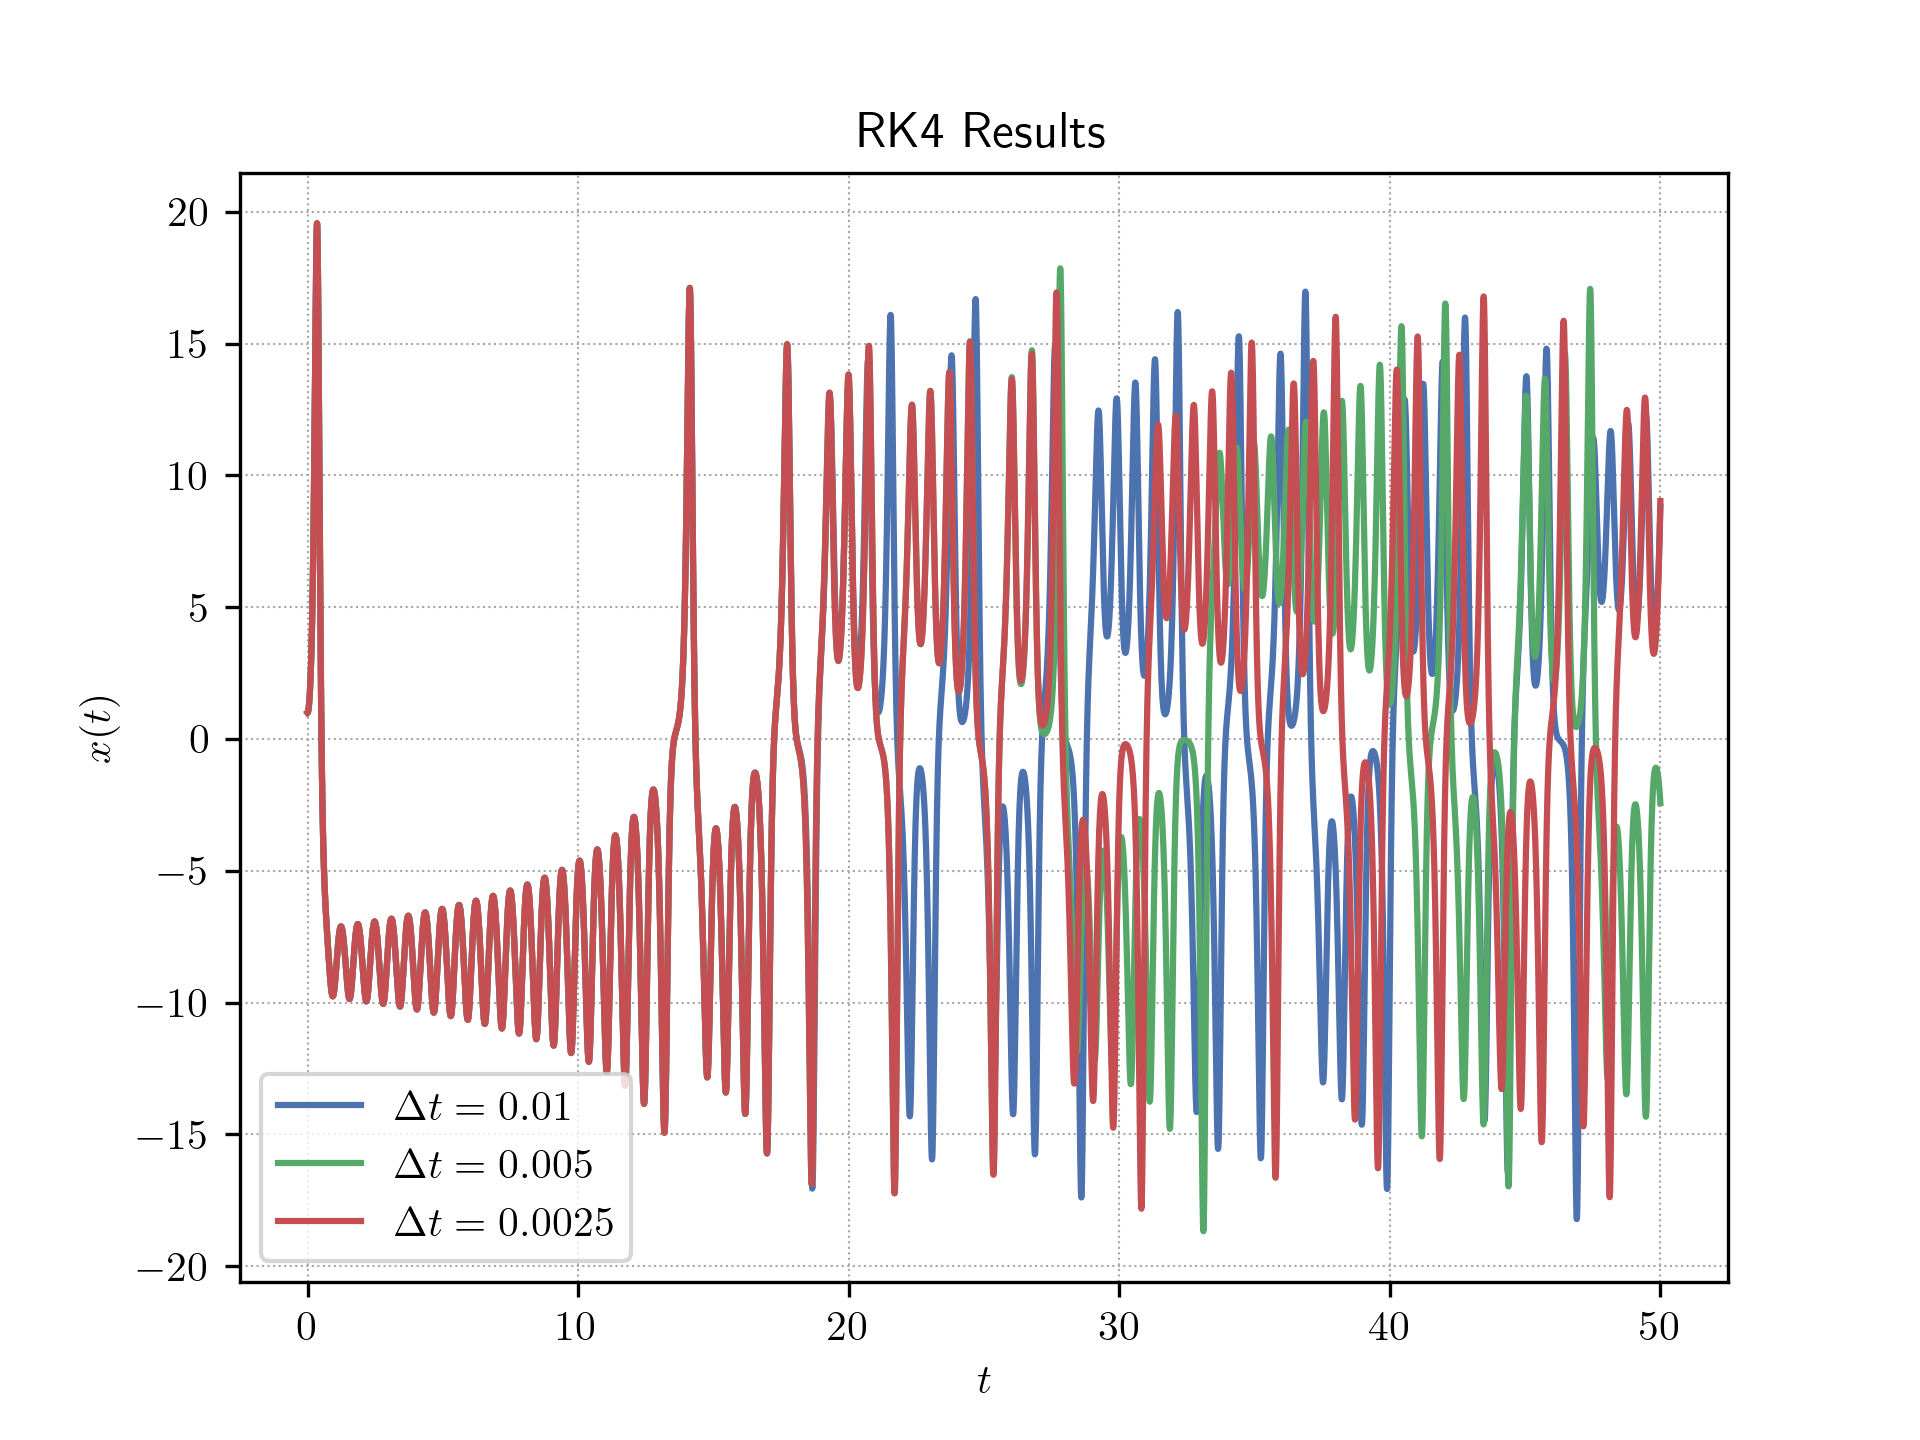
\includegraphics[width=0.75\textwidth]{../outputs/rk4_q2.png}

    Figure 2: SciPy's \texttt{solve\_ivp} results.

    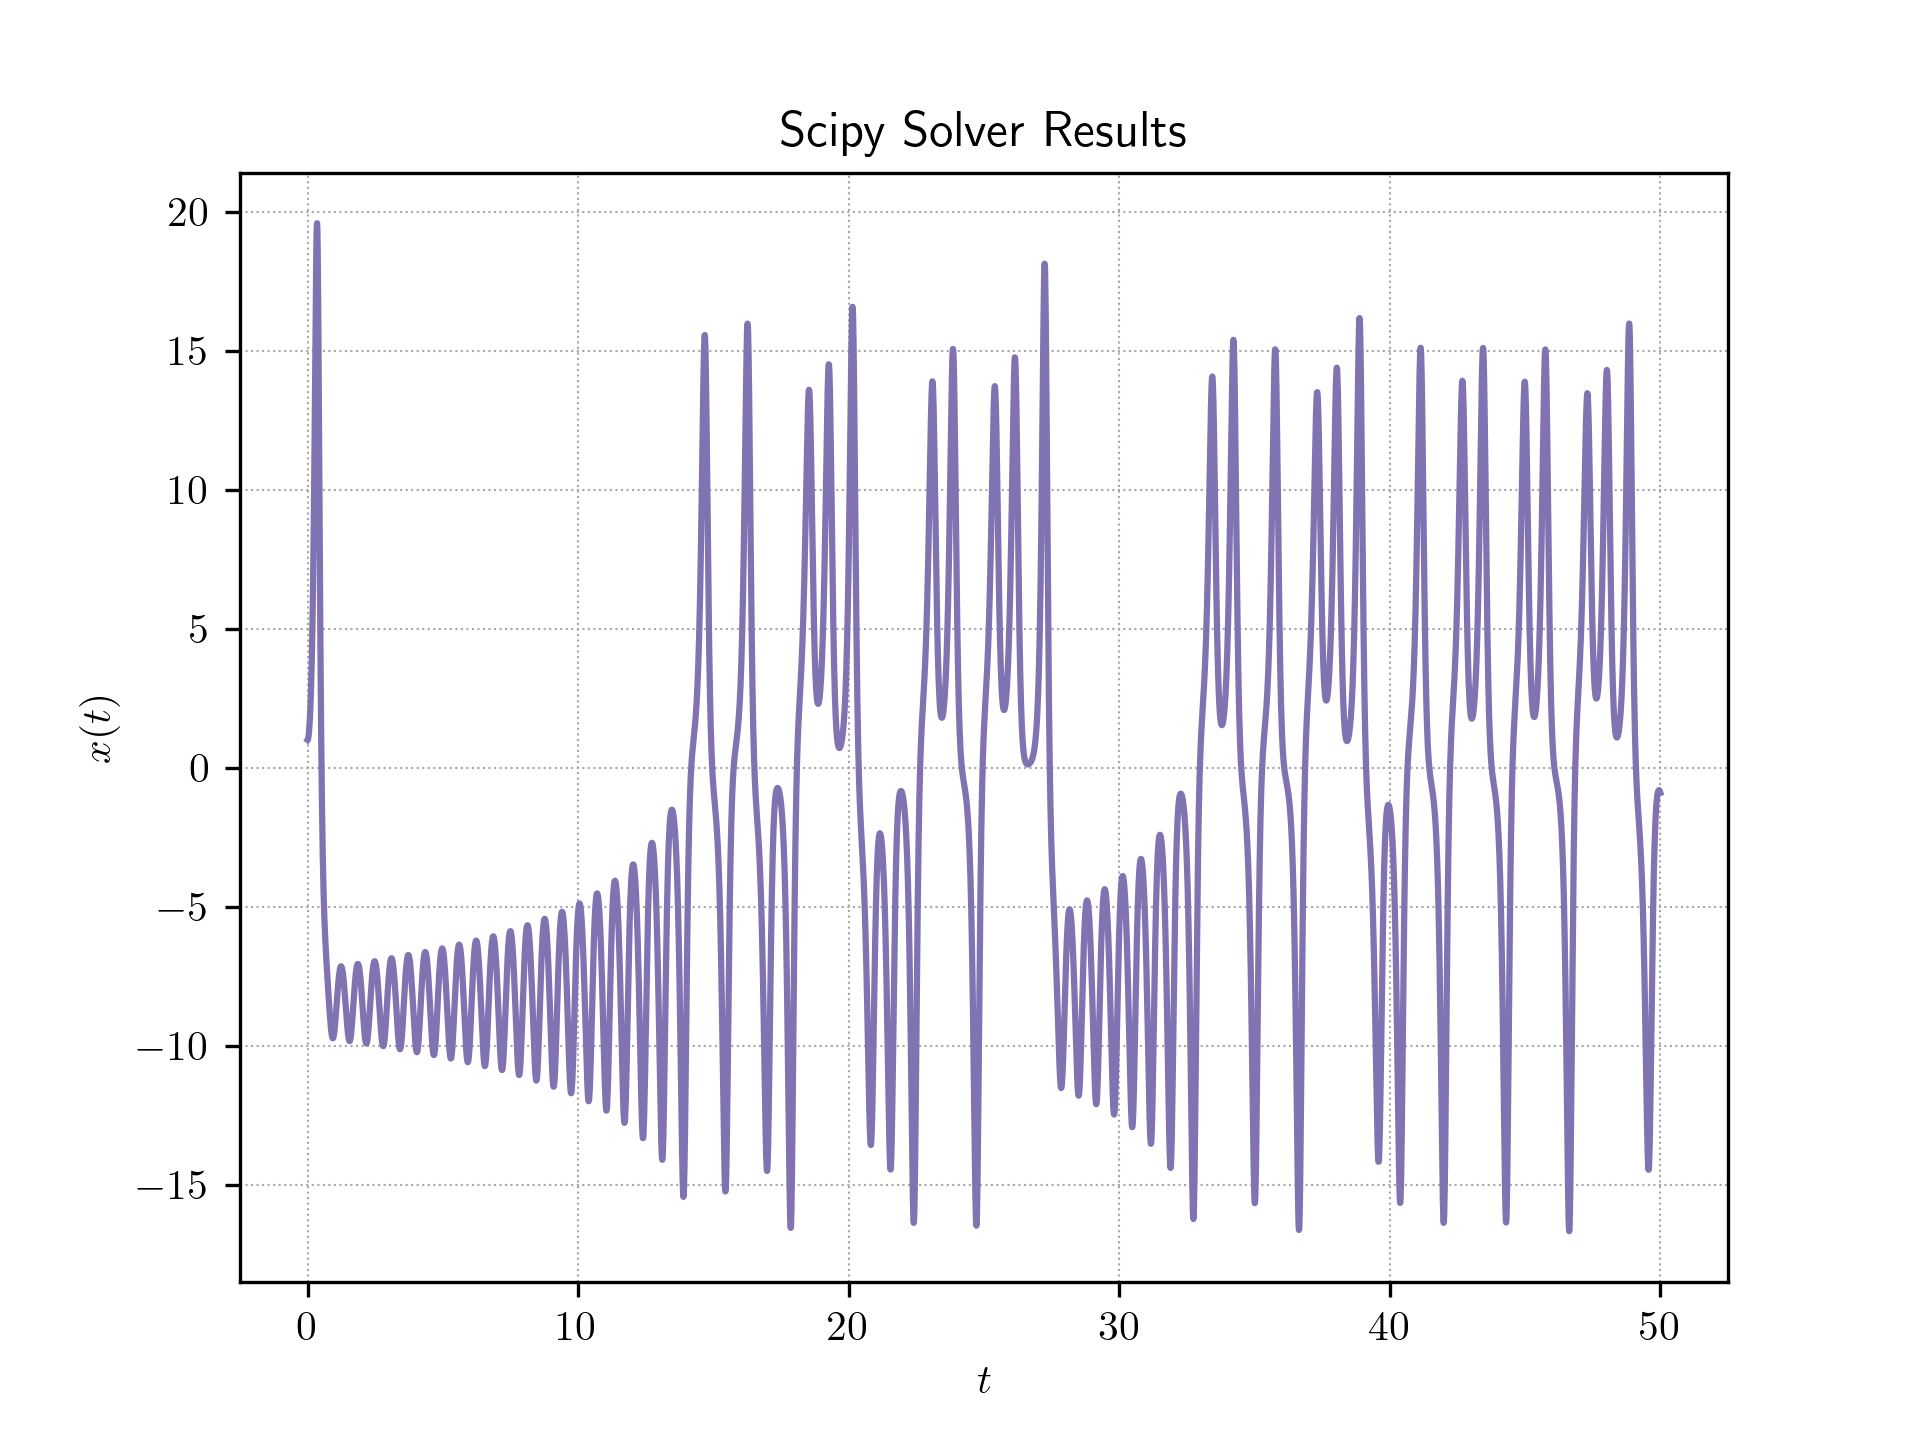
\includegraphics[width=0.75\textwidth]{../outputs/rk4_scipy.png}
\end{center}

\newpage
From Figure 1, we observe that as the time step $\Delta t$ decreases, the solution seems to converge to a more consistent trajectory for larger time intervals. Or in other words, we see that the overlap for trajectories with smaller times steps is better before the Lorenz system's chaotic nature causes divergence. 

In comparing Figures 1 and 2, we can see that the RK4 implementation closely matches the results from SciPy's \texttt{solve\_ivp} up until about $t\approx 13$ (when graphs are overlapped). After this point, the trajectories begin to diverge due to numerical differences. This behavior is expected as \texttt{solve\_ivp} uses an adaptive time-stepping method in comparison to our fixed time step RK4 implementation, which can lead to different numerical errors accumulating over time. However, since we observed that the initial trajectories match closely, we can conclude that our RK4 implementation is correct and captures the dynamics of the Lorenz system accurately for smaller time intervals.

\hrulefill

\question{Parameter Exploration}
Simulate $[0,T=50]$ for the following parameter sets:
\[\text{\textbf{Case A:}} (\sigma, \rho, \beta) = (10, 5, 8/3) \quad \text{\textbf{Case B:}} (\sigma, \rho, \beta) = (10, 15, 2)\]
\[\text{\textbf{Case C:}} (\sigma, \rho, \beta) = (10, 28, 8/3) \quad \text{\textbf{Case D:}} (\sigma, \rho, \beta) = (10, 40, 8/3)\]
For each case:
\begin{itemize}
    \item [a.] Plot $x(t)$, $y(t)$, and $z(t)$ vs. $t$ over $[0,T]$.
    \item [b.] Plot the trajectory $(x(t), y(t), z(t))$ in phase space.
    \item [c.] Comment on the behaviors of the system for each case.
\end{itemize}

\solution
temp text

\hrulefill

\question{Sensitivity Experiment (repeatability test)}
Choose one of the four parameter sets from Question 3. Run two simulations with the following initial conditions:
\[ (x_0, y_0, z_0) = (1, 1, 1) \quad (x_0, y_0, z_0) = (1 + 10^{-8}, 1, 1) \]
using the same $\Delta t$.
\begin{itemize}
    \item[a.] Plot $x(t)$ from both runs on the same graph. Comment on the results.
    \item[b.] Plot the difference $|x_1(t) - x_2(t)|$ vs. $t$ on a semilog-y plot (i.e., only the $y$-axis is logarithmic). Comment on the results.
    \item[c.] Do the Same for $y(t)$ and $z(t)$. 
\end{itemize}

\solution
temp text

\hrulefill

\question{Time Step Effects and Numerical Stability}
For Case D, repeat the computation with:
\[ \Delta t = 0.02, 0.01, 0.005\]
\begin{itemize}
    \item[a.] Compare the time series plots and the phase-space trajectories.
    \item[b.] Describe any visible artifacts (eg. drift, distortion of trajectories, blow-up) 
    \item[c.] Describe the influence of step size from the simulation results. 
\end{itemize}

\solution
dummy text

\end{document}